\srcpage{291}
\section*{第13章\quad 拟阵}\addcontentsline{toc}{section}{第13章\quad 拟阵}
许多组合优化问题可表述如下：给定一个集合系统 $(E,\F)$，个即有限集 $E$ 及某 $\F\subseteq2^E$，再给定费用函数 $c:\F\to\R$，求 $\F$ 中费用最小或最大的元素。下面考虑模函数 $c$，即对所有 $X\subseteq E$ 假定
\[c(X)=c(\varnothing)+\sum_{x\in X}\bigl(c(\{x\})-c(\varnothing)\bigr).\]
等价地，给定函数 $c:E\to\R$，并记 $c(X)=\sum_{e\in X}c(e)$。

本章只考虑 $\F$ 描述独立系统（即对子集封闭）乃至拟阵的组合优化问题。本章的结果推广了前面若干章得到的结论。

第13.1节引入独立系统和拟阵，并说明许多组合优化问题可在这一框架中描述。拟阵有若干等价的公理系统（第13.2节），以及一种有趣的对偶关系（第13.3节）。拟阵之所以重要，主要在于可以用简单的贪心算法在拟阵上进行优化。第13.4节分析贪心算法，随后转向两个拟阵之交上的优化问题。第13.5和13.7节说明此问题可在多项式时间内求解。这也解决了以独立集覆盖一个拟阵的问题，见第13.6节。

\sect{13.1\quad 独立系统与拟阵}
\st{定义13.1} 若集合系统 $(E,\F)$ 满足下列条件，就称其为\textbf{独立系统}（independence system）：
\begin{description}
\item[(M1)] $\varnothing\in\F$；
\item[(M2)] 若 $X\subseteq Y\in\F$，则 $X\in\F$。
\end{description}
$\F$ 的元素称为\textbf{独立集}，$2^E\setminus\F$ 的元素称为\textbf{相关集}。极小相关集称为\textbf{回路}（circuit），极大独立集称为\textbf{基}（basis）。对 $X\subseteq E$，$X$ 的极大独立子集称为 $X$ 的基。

\st{定义13.2} 设 $(E,\F)$ 是独立系统。对 $X\subseteq E$，定义 $X$ 的\textbf{秩}为
\[r(X):=\max\{|Y|:Y\subseteq X,\ Y\in\F\}.\]
并定义 $X$ 的\textbf{闭包}为 $\sigma(X):=\{y\in E:r(X\cup\{y\})=r(X)\}$。

\srcpage{292}
本章始终以 $(E,\F)$ 表示独立系统，以 $c:E\to\R$ 表示费用函数。我们着重考虑以下两个问题。
\alg{独立系统上的最大化问题}
\textbf{实例：}独立系统 $(E,\F)$ 和函数 $c:E\to\R$。\par
\textbf{任务：}求 $X\in\F$，使 $c(X):=\sum_{e\in X}c(e)$ 最大。
\alg{独立系统上的最小化问题}
\textbf{实例：}独立系统 $(E,\F)$ 和函数 $c:E\to\R$。\par
\textbf{任务：}求一个基 $B$，使 $c(B)$ 最小。

这里对实例的说明还不十分精确。集合 $E$ 和费用函数 $c$ 像通常一样显式给出。但 $\F$ 通常并不通过列出其全部元素来给出，而是假定有一个预言机：给定 $F\subseteq E$，它能判定 $F\in\F$ 是否成立。第13.4节将再次讨论这个问题。

下面的例子表明，许多组合优化问题确实具有上述两种形式之一。
\begin{enumerate}[label=(\arabic*)]
\item \textbf{最大权稳定集问题。}给定图 $G$ 及权函数 $c:V(G)\to\R$，求 $G$ 中权重最大的稳定集 $X$。这里 $E=V(G)$，$\F=\{F\subseteq E:F\text{ 在 }G\text{ 中稳定}\}$。
\item \textbf{旅行商问题（TSP）。}给定完全无向图 $G$ 及权函数 $c:E(G)\to\R_+$，求 $G$ 中权重最小的哈密顿回路。这里 $E=E(G)$，$\F=\{F\subseteq E:F\text{ 是 }G\text{ 中某个哈密顿回路的子集}\}$。
\item \textbf{最短路问题。}给定有向图 $G$、$c:E(G)\to\R$ 以及 $s,t\in V(G)$，且 $t$ 从 $s$ 可达，求关于 $c$ 的最短 $s$--$t$ 路。这里 $E=E(G)$，$\F=\{F\subseteq E:F\text{ 是某条 }s\text{--}t\text{ 路的子集}\}$。
\item \textbf{背包问题。}给定非负数 $n,c_i,w_i$（$1\le i\le n$）及 $W$，求 $S\subseteq\{1,\ldots,n\}$，使 $\sum_{j\in S}w_j\le W$，且 $\sum_{j\in S}c_j$ 最大。这里
\[E=\{1,\ldots,n\},\qquad\F=\left\{F\subseteq E:\sum_{j\in F}w_j\le W\right\}.\]
\item \textbf{最小生成树问题。}给定连通无向图 $G$ 及权函数 $c:E(G)\to\R$，求 $G$ 的最小权生成树。这里 $E=E(G)$，$\F$ 是 $G$ 中森林的全体。
\item \textbf{最大权森林问题。}给定无向图 $G$ 及权函数 $c:E(G)\to\R$，求 $G$ 中的最大权森林。这里同样 $E=E(G)$，$\F$ 是 $G$ 中森林的全体。
\end{enumerate}

\srcpage{293}
\begin{enumerate}[label=(\arabic*),start=7]
\item \textbf{斯坦纳树问题。}给定连通无向图 $G$、权函数 $c:E(G)\to\R_+$ 和终端集 $T\subseteq V(G)$，求 $T$ 的斯坦纳树，即满足 $T\subseteq V(S)$、$E(S)\subseteq E(G)$ 的树 $S$，使 $c(E(S))$ 最小。这里 $E=E(G)$，$\F=\{F\subseteq E:F\text{ 是 }T\text{ 的某棵斯坦纳树的子集}\}$。
\item \textbf{最大权分支问题。}给定有向图 $G$ 及权函数 $c:E(G)\to\R$，求 $G$ 中的最大权分支。这里 $E=E(G)$，$\F$ 是 $G$ 中分支的全体。
\item \textbf{最大权匹配问题。}给定无向图 $G$ 及权函数 $c:E(G)\to\R$，求 $G$ 中的最大权匹配。这里 $E=E(G)$，$\F$ 是 $G$ 中匹配的全体。
\end{enumerate}
这份列表既包含 NP 困难问题（(1)、(2)、(4)、(7)），也包含可在多项式时间内求解的问题（(5)、(6)、(8)、(9)）。问题(3)按上述形式是 NP 困难的，但当权重非负时可在多项式时间内求解（见第15章）。

\st{定义13.3} 若独立系统还满足下列条件，就称它为\textbf{拟阵}（matroid）：
\begin{description}\item[(M3)] 若 $X,Y\in\F$ 且 $|X|>|Y|$，则存在 $x\in X\setminus Y$，使 $Y\cup\{x\}\in\F$。\end{description}
matroid 这一名称表明这种结构是矩阵的推广。第一个例子将说明这一点。

\st{命题13.4} 以下独立系统 $(E,\F)$ 都是拟阵：
\begin{enumerate}[label=(\alph*)]
\item $E$ 是某个域上矩阵 $A$ 的列的集合，$\F:=\{F\subseteq E:F\text{ 中的列在该域上线性无关}\}$。
\item $E$ 是某个无向图 $G$ 的边集，$\F:=\{F\subseteq E:(V(G),F)\text{ 是森林}\}$。
\item $E$ 是有限集，$k$ 是整数，$\F:=\{F\subseteq E:|F|\le k\}$。
\item $E$ 是某个无向图 $G$ 的边集，$S$ 是 $G$ 中的稳定集，$k_s$（$s\in S$）是整数，$\F:=\{F\subseteq E:|\delta_F(s)|\le k_s\text{ 对所有 }s\in S\}$。
\item $E$ 是某个有向图 $G$ 的边集，$S\subseteq V(G)$，$k_s$（$s\in S$）是整数，$\F:=\{F\subseteq E:|\delta^-_F(s)|\le k_s\text{ 对所有 }s\in S\}$。
\end{enumerate}
\pr 各种情形下 $(E,\F)$ 显然都是独立系统，只需验证(M3)。(a)是线性代数中的熟知结论，(c)显然成立。

对(b)，设 $X,Y\in\F$，并假设每个 $x\in X\setminus Y$ 都满足 $Y\cup\{x\}\notin\F$。我们证明 $|X|\le|Y|$。对每条边 $x=\{v,w\}\in X$，$v,w$ 位于 $(V(G),Y)$ 的同一连通分支中。因此 $(V(G),X)$ 的每个连通分支 $Z\subseteq V(G)$ 都包含在 $(V(G),Y)$ 的某个连通分支中。所以森林 $(V(G),X)$ 的连通分支数 $p$ 不小于森林 $(V(G),Y)$ 的连通分支数 $q$。于是 $|V(G)|-|X|=p\ge q=|V(G)|-|Y|$，从而 $|X|\le|Y|$。

\srcpage{294}
为验证(d)中的(M3)，设 $X,Y\in\F$ 且 $|X|>|Y|$。令 $S':=\{s\in S:|\delta_Y(s)|=k_s\}$。由于 $|X|>|Y|$，且对所有 $s\in S'$ 都有 $|\delta_X(s)|\le k_s$，存在 $e\in X\setminus Y$，使得对所有 $s\in S'$ 都有 $e\notin\delta(s)$。于是 $Y\cup\{e\}\in\F$。

(e)的证明相同，只需将 $\delta$ 换成 $\delta^-$。\qed
其中一些拟阵有专门名称：(a)中的拟阵称为 $A$ 的\textbf{向量拟阵}。设 $M$ 是拟阵。如果域 $\mathbb F$ 上存在矩阵 $A$，使 $M$ 是 $A$ 的向量拟阵，就称 $M$ 在 $\mathbb F$ 上\textbf{可表示}。有些拟阵在任何域上都不可表示。

(b)中的拟阵称为 $G$ 的\textbf{圈拟阵}，有时记作 $M(G)$。若一个拟阵是某个图的圈拟阵，就称它为\textbf{图拟阵}。(c)中的拟阵称为\textbf{均匀拟阵}。

本节开头所列的独立系统中，只有(5)和(6)中的图拟阵是拟阵。借助下述定理，很容易验证其余独立系统一般都不是拟阵（习题1）。
\st{定理13.5} 设 $(E,\F)$ 是独立系统。以下命题等价：
\begin{description}
\item[(M3)] 若 $X,Y\in\F$ 且 $|X|>|Y|$，则存在 $x\in X\setminus Y$，使 $Y\cup\{x\}\in\F$。
\item[(M3$'$)] 若 $X,Y\in\F$ 且 $|X|=|Y|+1$，则存在 $x\in X\setminus Y$，使 $Y\cup\{x\}\in\F$。
\item[(M3$''$)] 对每个 $X\subseteq E$，$X$ 的所有基具有相同的基数。
\end{description}
\pr (M3)$\Leftrightarrow$(M3$'$)及(M3)$\Rightarrow$(M3$''$)显然成立。证明(M3$''$)$\Rightarrow$(M3)：设 $X,Y\in\F$ 且 $|X|>|Y|$。由(M3$''$)，$Y$ 不可能是 $X\cup Y$ 的基。因此必存在 $x\in(X\cup Y)\setminus Y=X\setminus Y$，使 $Y\cup\{x\}\in\F$。\qed
有时引入第二个秩函数很有用。
\st{定义13.6} 设 $(E,\F)$ 是独立系统。对 $X\subseteq E$，定义\textbf{下秩}为
\[\rho(X):=\min\{|Y|:Y\subseteq X,\ Y\in\F,\ \text{且对所有 }x\in X\setminus Y,\ Y\cup\{x\}\notin\F\}.\]
$(E,\F)$ 的\textbf{秩商}定义为
\[q(E,\F):=\min_{F\subseteq E}\frac{\rho(F)}{r(F)}.\]
\st{命题13.7} 设 $(E,\F)$ 是独立系统，则 $q(E,\F)\le1$。此外，$(E,\F)$ 是拟阵当且仅当 $q(E,\F)=1$。
\pr 不等式 $q(E,\F)\le1$ 直接来自定义。$q(E,\F)=1$ 显然与(M3$''$)等价。\qed
估计秩商时可以使用下述结论。
\srcpage{295}
\st{定理13.8（Hausmann、Jenkyns 和 Korte [1980]）} 设 $(E,\F)$ 是独立系统。如果对任意 $A\in\F$ 和 $e\in E$，$A\cup\{e\}$ 至多包含 $p$ 个回路，那么 $q(E,\F)\ge1/p$。
\pr 设 $F\subseteq E$，$J,K$ 是 $F$ 的两个基。我们证明 $|J|/|K|\ge1/p$。
令 $J\setminus K=\{e_1,\ldots,e_t\}$。构造 $J\cup K$ 的独立子集序列 $K=K_0,K_1,\ldots,K_t$，使 $J\cap K\subseteq K_i$、$K_i\cap\{e_1,\ldots,e_t\}=\{e_1,\ldots,e_i\}$，且对 $i=1,\ldots,t$ 有 $|K_{i-1}\setminus K_i|\le p$。
由于 $K_i\cup\{e_{i+1}\}$ 至多包含 $p$ 个回路，且每个回路必与 $K_i\setminus J$ 相交（因为 $J$ 独立），存在 $X\subseteq K_i\setminus J$，满足 $|X|\le p$ 且 $(K_i\setminus X)\cup\{e_{i+1}\}\in\F$。令 $K_{i+1}:=(K_i\setminus X)\cup\{e_{i+1}\}$。
现在 $J\subseteq K_t\in\F$。因为 $J$ 是 $F$ 的基，故 $J=K_t$。于是
\[|K\setminus J|=\sum_{i=1}^t|K_{i-1}\setminus K_i|\le pt=p|J\setminus K|,\]
从而 $|K|\le p|J|$。\qed
这说明例(9)中 $q(E,\F)\ge1/2$（另见第10章习题1）。事实上，当且仅当 $G$ 含有一条长度为3的路作为子图时，$q(E,\F)=1/2$；否则 $q(E,\F)=1$。列表中例(1)的秩商可以任意小（取 $G$ 为星图）。习题5将讨论其他独立系统的秩商。
\sect{13.2\quad 拟阵的其他公理}
本节讨论定义拟阵的其他公理系统。它们刻画拟阵的基族、秩函数、闭包算子和回路族的基本性质。
\st{定理13.9} 设 $E$ 是有限集，$\B\subseteq2^E$。$\B$ 是某个拟阵 $(E,\F)$ 的基的集合，当且仅当：
\begin{description}
\item[(B1)] $\B\ne\varnothing$；
\item[(B2)] 对任意 $B_1,B_2\in\B$ 和 $x\in B_1\setminus B_2$，存在 $y\in B_2\setminus B_1$，使 $(B_1\setminus\{x\})\cup\{y\}\in\B$。
\end{description}
\pr 拟阵的基族满足(B1)（由(M1)）和(B2)：对基 $B_1,B_2$ 及 $x\in B_1\setminus B_2$，$B_1\setminus\{x\}$ 独立。由(M3)，存在 $y\in B_2\setminus B_1$，使 $(B_1\setminus\{x\})\cup\{y\}$ 独立。由于拟阵所有基的基数相同，该集合必为基。
反之，设 $\B$ 满足(B1)、(B2)。首先证明 $\B$ 的所有元素基数相同。否则取 $B_1,B_2\in\B$，使 $|B_1|>|B_2|$ 且 $|B_1\cap B_2|$ 最大。取 $x\in B_1\setminus B_2$。由(B2)，存在 $y\in B_2\setminus B_1$，使 $(B_1\setminus\{x\})\cup\{y\}\in\B$，这与交集基数的最大性矛盾。

\srcpage{296}
现在令 $\F:=\{F\subseteq E:\text{存在 }B\in\B\text{ 使 }F\subseteq B\}$。则 $(E,\F)$ 是独立系统，$\B$ 是它的基族。为验证(M3)，设 $X,Y\in\F$ 且 $|X|>|Y|$。取 $X\subseteq B_1\in\B$、$Y\subseteq B_2\in\B$，并使 $|B_1\cap B_2|$ 最大。若 $B_2\cap(X\setminus Y)\ne\varnothing$，便可扩充 $Y$，证明即告完成。
我们断言另一种情形 $B_2\cap(X\setminus Y)=\varnothing$ 不可能发生。在此假设下，
\begin{align*}
|B_1\cap B_2|+|Y\setminus B_1|+|(B_2\setminus B_1)\setminus Y|
&=|B_2|=|B_1|\\&\ge|B_1\cap B_2|+|X\setminus Y|.
\end{align*}
由于 $|X\setminus Y|>|Y\setminus X|\ge|Y\setminus B_1|$，可得 $(B_2\setminus B_1)\setminus Y\ne\varnothing$。取其中的 $y$。由(B2)，存在 $x\in B_1\setminus B_2$，使 $(B_2\setminus\{y\})\cup\{x\}\in\B$，与 $|B_1\cap B_2|$ 的最大性矛盾。\qed
拟阵的一条极重要性质是：它的秩函数是次模的。
\st{定理13.10} 设 $E$ 是有限集，$r:2^E\to\Z_+$。下列命题等价：
\begin{enumerate}[label=(\alph*)]
\item $r$ 是某个拟阵 $(E,\F)$ 的秩函数，且 $\F=\{F\subseteq E:r(F)=|F|\}$。
\item 对所有 $X,Y\subseteq E$，有
\begin{description}
\item[(R1)] $r(X)\le|X|$；
\item[(R2)] 若 $X\subseteq Y$，则 $r(X)\le r(Y)$；
\item[(R3)] $r(X\cup Y)+r(X\cap Y)\le r(X)+r(Y)$。
\end{description}
\item 对所有 $X\subseteq E$ 和 $x,y\in E$，有
\begin{description}
\item[(R1$'$)] $r(\varnothing)=0$；
\item[(R2$'$)] $r(X)\le r(X\cup\{y\})\le r(X)+1$；
\item[(R3$'$)] 若 $r(X\cup\{x\})=r(X\cup\{y\})=r(X)$，则 $r(X\cup\{x,y\})=r(X)$。
\end{description}
\end{enumerate}
\pr (a)$\Rightarrow$(b)：独立系统的秩函数显然满足(R1)、(R2)。若为拟阵，还能证明(R3)：设 $A$ 是 $X\cap Y$ 的一个基。由(M3)，可将 $A$ 扩充为 $X$ 的基 $A\mathbin{\dot\cup}B$，再扩充为 $X\cup Y$ 的基 $(A\cup B)\mathbin{\dot\cup}C$。则 $A\cup C$ 是 $Y$ 的独立子集，故
\begin{align*}
r(X)+r(Y)&\ge|A\cup B|+|A\cup C|\\
&=2|A|+|B|+|C|=|A\cup B\cup C|+|A|\\
&=r(X\cup Y)+r(X\cap Y).
\end{align*}
(b)$\Rightarrow$(c)：(R1)蕴含(R1$'$)，(R2)蕴含 $r(X)\le r(X\cup\{y\})$。由(R3)、(R1)，
\[r(X\cup\{y\})\le r(X)+r(\{y\})-r(X\cap\{y\})\le r(X)+r(\{y\})\le r(X)+1,\]
这就证明了(R2$'$)。

\srcpage{297}
当 $x=y$ 时(R3$'$)显然成立。若 $x\ne y$，由(R2)、(R3)，
\[2r(X)\le r(X)+r(X\cup\{x,y\})\le r(X\cup\{x\})+r(X\cup\{y\}),\]
从而得到(R3$'$)。

(c)$\Rightarrow$(a)：设 $r:2^E\to\Z_+$ 满足(R1$'$)--(R3$'$)，令 $\F:=\{F\subseteq E:r(F)=|F|\}$。我们断言 $(E,\F)$ 是拟阵。(M1)来自(R1$'$)。由(R2$'$)，对所有 $X\subseteq E$ 有 $r(X)\le|X|$。若 $Y\in\F$、$y\in Y$，并令 $X:=Y\setminus\{y\}$，则
\[|X|+1=|Y|=r(Y)=r(X\cup\{y\})\le r(X)+1\le|X|+1,\]
所以 $X\in\F$，从而(M2)成立。

设 $X,Y\in\F$ 且 $|X|=|Y|+1$。令 $X\setminus Y=\{x_1,\ldots,x_k\}$。若(M3$'$)不成立，即对 $i=1,\ldots,k$ 有 $r(Y\cup\{x_i\})=|Y|$，则由(R3$'$)，对 $i=2,\ldots,k$ 有 $r(Y\cup\{x_1,x_i\})=r(Y)$。反复使用这一论证可得
\[r(Y)=r(Y\cup\{x_1,\ldots,x_k\})=r(X\cup Y)\ge r(X),\]
矛盾。因此 $(E,\F)$ 确实是拟阵。为证明 $r$ 是其秩函数，只需证明对所有 $X\subseteq E$，有 $r(X)=\max\{|Y|:Y\subseteq X,r(Y)=|Y|\}$。取 $X$ 中满足 $r(Y)=|Y|$ 的最大子集 $Y$。对每个 $x\in X\setminus Y$，有 $r(Y\cup\{x\})<|Y|+1$，故由(R2$'$)，$r(Y\cup\{x\})=|Y|$。反复应用(R3$'$)得 $r(X)=|Y|$。\qed

\st{定理13.11} 设 $E$ 是有限集，$\sigma:2^E\to2^E$ 是函数。$\sigma$ 是某个拟阵 $(E,\F)$ 的闭包算子，当且仅当对所有 $X,Y\subseteq E$ 和 $x,y\in E$，下列条件成立：
\begin{description}
\item[(S1)] $X\subseteq\sigma(X)$；
\item[(S2)] $X\subseteq Y\subseteq E$ 蕴含 $\sigma(X)\subseteq\sigma(Y)$；
\item[(S3)] $\sigma(X)=\sigma(\sigma(X))$；
\item[(S4)] 若 $y\notin\sigma(X)$ 且 $y\in\sigma(X\cup\{x\})$，则 $x\in\sigma(X\cup\{y\})$。
\end{description}
\pr 若 $\sigma$ 是拟阵的闭包算子，则(S1)显然成立。对 $X\subseteq Y$ 和 $z\in\sigma(X)$，由(R3)、(R2)，
\begin{align*}
r(X)+r(Y)&=r(X\cup\{z\})+r(Y)\\
&\ge r((X\cup\{z\})\cap Y)+r(X\cup\{z\}\cup Y)\\
&\ge r(X)+r(Y\cup\{z\}),
\end{align*}
所以 $z\in\sigma(Y)$，(S2)成立。反复应用(R3$'$)可得对所有 $X$ 有 $r(\sigma(X))=r(X)$，从而(S3)成立。
为证明(S4)，假设存在 $X,x,y$，满足 $y\notin\sigma(X)$、$y\in\sigma(X\cup\{x\})$、$x\notin\sigma(X\cup\{y\})$。于是 $r(X\cup\{y\})=r(X)+1$、$r(X\cup\{x,y\})=r(X\cup\{x\})$，且 $r(X\cup\{x,y\})=r(X\cup\{y\})+1$。因此 $r(X\cup\{x\})=r(X)+2$，与(R2$'$)矛盾。

\srcpage{298}
反之，设 $\sigma:2^E\to2^E$ 满足(S1)--(S4)，令
\[\F:=\{X\subseteq E:\text{对所有 }x\in X,\ x\notin\sigma(X\setminus\{x\})\}.\]
我们断言 $(E,\F)$ 是拟阵。(M1)显然成立。若 $X\subseteq Y\in\F$、$x\in X$，则 $x\notin\sigma(Y\setminus\{x\})\supseteq\sigma(X\setminus\{x\})$，所以 $X\in\F$，即(M2)成立。证明(M3)需用以下结论。

\textbf{断言：}若 $X\in\F$、$Y\subseteq E$ 且 $|X|>|Y|$，则 $X\nsubseteq\sigma(Y)$。
对 $|Y\setminus X|$ 归纳。若 $Y\subset X$，取 $x\in X\setminus Y$。由 $X\in\F$ 及(S2)，有 $x\notin\sigma(X\setminus\{x\})\supseteq\sigma(Y)$，故 $x\in X\setminus\sigma(Y)$。
若 $|Y\setminus X|>0$，取 $y\in Y\setminus X$。由归纳假设，存在 $x\in X\setminus\sigma(Y\setminus\{y\})$。若 $x\notin\sigma(Y)$，结论已得。否则由(S4)，$y\in\sigma((Y\setminus\{y\})\cup\{x\})$。由(S1)可得 $Y\subseteq\sigma((Y\setminus\{y\})\cup\{x\})$，再由(S2)、(S3)，
\[\sigma(Y)\subseteq\sigma((Y\setminus\{y\})\cup\{x\}).\]
对 $X$ 和 $(Y\setminus\{y\})\cup\{x\}$ 应用归纳假设（注意 $x\ne y$），得 $X\nsubseteq\sigma((Y\setminus\{y\})\cup\{x\})$，故 $X\nsubseteq\sigma(Y)$，断言成立。

现验证(M3)。设 $X,Y\in\F$ 且 $|X|>|Y|$，由断言可取 $x\in X\setminus\sigma(Y)$。对每个 $z\in Y\cup\{x\}$，有 $z\notin\sigma(Y\setminus\{z\})$，因为 $Y\in\F$ 且 $x\notin\sigma(Y)=\sigma(Y\setminus\{x\})$。由(S4)，$z\notin\sigma(Y\setminus\{z\})$ 和 $x\notin\sigma(Y)$ 蕴含
\[z\notin\sigma((Y\setminus\{z\})\cup\{x\})\supseteq\sigma((Y\cup\{x\})\setminus\{z\}).\]
因此 $Y\cup\{x\}\in\F$，(M3)成立。于是 $(E,\F)$ 是拟阵，记其秩函数为 $r$、闭包算子为 $\sigma'$。还需证明 $\sigma=\sigma'$。由定义，对所有 $X\subseteq E$，
\[\sigma'(X)=\{y\in E:r(X\cup\{y\})=r(X)\},\]
\[r(X)=\max\{|Y|:Y\subseteq X,\ \text{对所有 }y\in Y,\ y\notin\sigma(Y\setminus\{y\})\}.\]
先证 $\sigma'(X)\subseteq\sigma(X)$。取 $z\in\sigma'(X)\setminus X$，以及 $X$ 的基 $Y$。由于
\[r(Y\cup\{z\})\le r(X\cup\{z\})=r(X)=|Y|<|Y\cup\{z\}|,\]
存在 $y\in Y\cup\{z\}$，使 $y\in\sigma((Y\cup\{z\})\setminus\{y\})$。若 $y=z$，则 $z\in\sigma(Y)$；否则由(S4)及 $y\notin\sigma(Y\setminus\{y\})$，也得 $z\in\sigma(Y)$。再由(S2)，$z\in\sigma(X)$。结合(S1)，包含关系成立。
现设 $z\notin\sigma'(X)$，即 $r(X\cup\{z\})>r(X)$。取 $X\cup\{z\}$ 的基 $Y$。则 $z\in Y$，且 $|Y\setminus\{z\}|=|Y|-1=r(X\cup\{z\})-1=r(X)$，所以 $Y\setminus\{z\}$ 是 $X$ 的基。于是 $X\subseteq\sigma'(Y\setminus\{z\})\subseteq\sigma(Y\setminus\{z\})$，从而 $\sigma(X)\subseteq\sigma(Y\setminus\{z\})$。由于 $z\notin\sigma(Y\setminus\{z\})$，得到 $z\notin\sigma(X)$。\qed
\st{定理13.12} 设 $E$ 是有限集，$\Cc\subseteq2^E$。$\Cc$ 是某个独立系统 $(E,\F)$ 的回路集合，其中 $\F=\{F\subseteq E:\text{不存在 }C\in\Cc\text{ 使 }C\subseteq F\}$，当且仅当：
\begin{description}\item[(C1)] $\varnothing\notin\Cc$；\item[(C2)] 对任意 $C_1,C_2\in\Cc$，$C_1\subseteq C_2$ 蕴含 $C_1=C_2$。\end{description}

\srcpage{299}
此外，若 $\Cc$ 是独立系统 $(E,\F)$ 的回路集合，则下列命题等价：
\begin{description}
\item[(a)] $(E,\F)$ 是拟阵。
\item[(b)] 对任意 $X\in\F$ 和 $e\in E$，$X\cup\{e\}$ 至多包含一个回路。
\item[(C3)] 对任意不同的 $C_1,C_2\in\Cc$ 及 $e\in C_1\cap C_2$，存在 $C_3\in\Cc$，使 $C_3\subseteq(C_1\cup C_2)\setminus\{e\}$。
\item[(C3$'$)] 对任意 $C_1,C_2\in\Cc$、$e\in C_1\cap C_2$ 和 $f\in C_1\setminus C_2$，存在 $C_3\in\Cc$，使 $f\in C_3\subseteq(C_1\cup C_2)\setminus\{e\}$。
\end{description}
\pr 由定义，任何独立系统的回路族都满足(C1)、(C2)。若 $\Cc$ 满足(C1)，则 $(E,\F)$ 是独立系统；若还满足(C2)，则 $\Cc$ 正是这个独立系统的回路集合。

(a)$\Rightarrow$(C3$'$)：设 $\Cc$ 是拟阵的回路族，$C_1,C_2\in\Cc$，$e\in C_1\cap C_2$，$f\in C_1\setminus C_2$。两次应用(R3)，得
\begin{align*}
&|C_1|-1+r((C_1\cup C_2)\setminus\{e,f\})+|C_2|-1\\
&=r(C_1)+r((C_1\cup C_2)\setminus\{e,f\})+r(C_2)\\
&\ge r(C_1)+r((C_1\cup C_2)\setminus\{f\})+r(C_2\setminus\{e\})\\
&\ge r(C_1\setminus\{f\})+r(C_1\cup C_2)+r(C_2\setminus\{e\})\\
&=|C_1|-1+r(C_1\cup C_2)+|C_2|-1.
\end{align*}
故 $r((C_1\cup C_2)\setminus\{e,f\})=r(C_1\cup C_2)$。取 $(C_1\cup C_2)\setminus\{e,f\}$ 的基 $B$，则 $B\cup\{f\}$ 包含回路 $C_3$，且 $f\in C_3\subseteq(C_1\cup C_2)\setminus\{e\}$，符合要求。

(C3$'$)$\Rightarrow$(C3)：显然。

(C3)$\Rightarrow$(b)：若 $X\in\F$ 而 $X\cup\{e\}$ 包含两个回路 $C_1,C_2$，则(C3)蕴含 $(C_1\cup C_2)\setminus\{e\}\notin\F$。但该集合是 $X$ 的子集，矛盾。

(b)$\Rightarrow$(a)：由定理13.8及命题13.7可得。\qed
特别是性质(b)将经常使用。对 $X\in\F$ 和 $e\in E$，若 $X\cup\{e\}\notin\F$，用 $C(X,e)$ 表示 $X\cup\{e\}$ 中唯一的回路；若 $X\cup\{e\}\in\F$，则记 $C(X,e):=\varnothing$。
\sect{13.3\quad 对偶性}
对偶性是拟阵理论中的另一个基本概念。
\st{定义13.13} 设 $(E,\F)$ 是独立系统。定义它的\textbf{对偶}为 $(E,\F^*)$，其中
\[\F^*=\{F\subseteq E:\text{存在 }(E,\F)\text{ 的基 }B\text{ 使 }F\cap B=\varnothing\}.\]
显然，独立系统的对偶仍是独立系统。

\srcpage{300}
\st{命题13.14} $(E,\F^{**})=(E,\F)$。
\pr $F\in\F^{**}$ 当且仅当存在 $(E,\F^*)$ 的基 $B^*$ 使 $F\cap B^*=\varnothing$；当且仅当存在 $(E,\F)$ 的基 $B$ 使 $F\cap(E\setminus B)=\varnothing$；当且仅当 $F\in\F$。\qed
\st{定理13.15} 设 $(E,\F)$ 是独立系统，$(E,\F^*)$ 是其对偶，$r,r^*$ 为相应的秩函数。
\begin{enumerate}[label=(\alph*)]
\item $(E,\F)$ 是拟阵当且仅当 $(E,\F^*)$ 是拟阵。（Whitney [1935]）
\item 若 $(E,\F)$ 是拟阵，则对 $F\subseteq E$，$r^*(F)=|F|+r(E\setminus F)-r(E)$。
\end{enumerate}
\pr 由命题13.14，只需证明(a)的一个方向。设 $(E,\F)$ 是拟阵，定义 $q:2^E\to\Z_+$，$q(F):=|F|+r(E\setminus F)-r(E)$。断言 $q$ 满足(R1)、(R2)、(R3)。由此及定理13.10，$q$ 是某个拟阵的秩函数。显然 $q(F)=|F|$ 当且仅当 $F\in\F^*$，所以 $q=r^*$，(a)、(b)即得证。

现证断言。由于 $r$ 满足(R2)，$q$ 满足(R1)。为验证 $q$ 满足(R2)，设 $X\subseteq Y\subseteq E$。由于 $(E,\F)$ 是拟阵，$r$ 满足(R3)，于是
\[r(E\setminus X)+0=r((E\setminus Y)\cup(Y\setminus X))+r(\varnothing)
\le r(E\setminus Y)+r(Y\setminus X).\]
从而
\[r(E\setminus X)-r(E\setminus Y)\le r(Y\setminus X)\le|Y\setminus X|=|Y|-|X|\]
（注意 $r$ 满足(R1)），故 $q(X)\le q(Y)$。

最后证明 $q$ 满足(R3)。设 $X,Y\subseteq E$。利用 $r$ 的(R3)，
\begin{align*}
q(X\cup Y)+q(X\cap Y)
&=|X\cup Y|+|X\cap Y|\\
&\quad+r(E\setminus(X\cup Y))+r(E\setminus(X\cap Y))-2r(E)\\
&=|X|+|Y|+r((E\setminus X)\cap(E\setminus Y))\\
&\quad+r((E\setminus X)\cup(E\setminus Y))-2r(E)\\
&\le|X|+|Y|+r(E\setminus X)+r(E\setminus Y)-2r(E)\\
&=q(X)+q(Y).
\end{align*}\qed
对任意图 $G$，前面引入了圈拟阵 $M(G)$，它当然有对偶。对给定平面嵌入的平面图 $G$，还有平面对偶 $G^*$（一般依赖于嵌入）。有趣的是，这两种对偶概念彼此一致。
\st{定理13.16} 设 $G$ 是具有任意平面嵌入的连通平面图，$G^*$ 是其平面对偶。那么
\[M(G^*)=(M(G))^*.\]
\srcpage{301}
\pr 对 $T\subseteq E(G)$，记 $\overline T^{\,*}:=\{e^*:e\in E(G)\setminus T\}$，其中 $e^*$ 是边 $e$ 的对偶边。需证明如下断言：$T$ 是 $G$ 的一棵生成树的边集，当且仅当 $\overline T^{\,*}$ 是 $G^*$ 的一棵生成树的边集。

由于 $(G^*)^*=G$（命题2.42），且对上述取对偶补集的操作再做一次会得到 $T$，只需证明一个方向。设 $\overline T^{\,*}$ 是 $G^*$ 的一棵生成树的边集。$(V(G),T)$ 必连通，否则一个连通分支会定义一个割，其对偶在 $\overline T^{\,*}$ 中包含一个圈（定理2.43）。另一方面，若 $(V(G),T)$ 包含一个圈，则其对偶边集构成割，使 $(V(G^*),\overline T^{\,*})$ 不连通。因此 $(V(G),T)$ 确实是 $G$ 的生成树。\qed
这说明，若 $G$ 平面，则 $(M(G))^*$ 是图拟阵。对任意图 $G$，若 $(M(G))^*$ 是图拟阵，例如 $(M(G))^*=M(G')$，则 $G'$ 显然是 $G$ 的抽象对偶。由第2章习题34，反过来也成立：$G$ 平面当且仅当 $G$ 有抽象对偶（Whitney [1933]）。于是 $(M(G))^*$ 是图拟阵当且仅当 $G$ 平面。

注意定理13.16相当直接地蕴含欧拉公式（定理2.32）。设 $G$ 是具有平面嵌入的连通平面图，$M(G)$ 是其圈拟阵。由定理13.15(b)，$r(E(G))+r^*(E(G))=|E(G)|$。因为 $r(E(G))=|V(G)|-1$（生成树的边数），且由定理13.16，$r^*(E(G))=|V(G^*)|-1$，可得 $G$ 的面数为 $|V(G^*)|=|E(G)|-|V(G)|+2$，即欧拉公式。

独立系统的对偶性在多面体组合学中也有一些很好的应用。若对任意 $X,Y\in\F$ 都有 $X\not\subset Y$，则称集合系统 $(E,\F)$ 为\textbf{杂族}（clutter）。其\textbf{阻塞杂族}定义为
\[\operatorname{BL}(E,\F):=(E,\{X\subseteq E:X\cap Y\ne\varnothing\text{ 对所有 }Y\in\F,
\ X\text{ 对此性质极小}\}).\]
对独立系统 $(E,\F)$ 及其对偶 $(E,\F^*)$，分别以 $\B,\B^*$ 表示基族，以 $\Cc,\Cc^*$ 表示回路族。（除 $\F=\varnothing$ 或 $\F=\{\varnothing\}$ 外，每个杂族都能以这两种方式出现。）由定义立得 $(E,\B^*)=\operatorname{BL}(E,\Cc)$，$(E,\Cc^*)=\operatorname{BL}(E,\B)$。结合命题13.14，对任意杂族 $(E,\F)$，
\[\operatorname{BL}(\operatorname{BL}(E,\F))=(E,\F).\]
下面列举杂族 $(E,\F)$ 及其阻塞杂族 $(E,\F')$。每例中 $E=E(G)$，$G$ 是某个图：
\begin{enumerate}[label=(\arabic*)]
\item $\F$ 是生成树全体，$\F'$ 是极小割全体；
\item $\F$ 是以 $r$ 为根的树形图全体，$\F'$ 是极小 $r$-割全体；
\item $\F$ 是 $s$--$t$ 路全体，$\F'$ 是分离 $s,t$ 的极小割全体（无向图、有向图均适用）；
\item $\F$ 是无向图中圈的全体，$\F'$ 是极大森林的补集全体；
\item $\F$ 是有向图中有向圈的全体，$\F'$ 是极小反馈边集全体；
\end{enumerate}

\srcpage{302}
\begin{enumerate}[label=(\arabic*),start=6]
\item $\F$ 是收缩后能使有向图变为强连通的极小边集全体，$\F'$ 是极小有向割全体；
\item $\F$ 是极小 $T$-连接全体，$\F'$ 是极小 $T$-割全体。
\end{enumerate}
这些阻塞关系都易于验证：(1)、(2)直接由定理2.4、2.5得到；(3)、(4)、(5)显然；(6)来自推论2.7，(7)来自命题12.6。

在某些情形下，阻塞杂族为非负费用函数下的独立系统最小化问题给出了多面体刻画。
\st{定义13.17} 设 $(E,\F)$ 为杂族，$(E,\F')$ 是其阻塞杂族，$P$ 是 $\F$ 各元素的关联向量的凸包。若
\[\{x+y:x\in P,y\in\R_+^E\}
=\left\{x\in\R_+^E:\sum_{e\in B}x_e\ge1\text{ 对所有 }B\in\F'\right\},\]
则称 $(E,\F)$ 具有\textbf{最大流最小割性质}。
上述列表中的(2)、(7)是例子（定理6.14、12.16），(3)、(6)也是（见习题10）。下述定理将这一覆盖型表述与对偶问题的打包型表述联系起来，因而能由一些极小极大定理推出另一些极小极大定理。
\st{定理13.18（Fulkerson [1971]、Lehman [1979]）} 设 $(E,\F)$ 为杂族，$(E,\F')$ 是其阻塞杂族。下列命题等价：
\begin{enumerate}[label=(\alph*)]
\item $(E,\F)$ 具有最大流最小割性质；
\item $(E,\F')$ 具有最大流最小割性质；
\item 对每个 $c:E\to\R_+$，有
\[\min\{c(A):A\in\F\}=\max\left\{\one y:y\in\R_+^{\F'},\ \sum_{\substack{B\in\F'\\e\in B}}y_B\le c(e)\text{ 对所有 }e\in E\right\}.\]
\end{enumerate}
\pr 由于 $\operatorname{BL}(E,\F')=\operatorname{BL}(\operatorname{BL}(E,\F))=(E,\F)$，只需证明(a)$\Rightarrow$(c)$\Rightarrow$(b)；交换 $\F$ 与 $\F'$ 即得(b)$\Rightarrow$(a)。

(a)$\Rightarrow$(c)：由推论3.28，对每个 $c:E\to\R_+$，
\[\min\{c(A):A\in\F\}=\min\{cx:x\in P\}=\min\{c(x+y):x\in P,y\in\R_+^E\},\]
其中 $P$ 是 $\F$ 各元素关联向量的凸包。结合最大流最小割性质和线性规划对偶定理3.16，得到(c)。

(c)$\Rightarrow$(b)：以 $P'$ 表示 $\F'$ 各元素关联向量的凸包。需证明
\[\{x+y:x\in P',y\in\R_+^E\}=\left\{x\in\R_+^E:\sum_{e\in A}x_e\ge1\text{ 对所有 }A\in\F\right\}.\]
由阻塞杂族的定义，“$\subseteq$”显然。只需证反向包含。设 $c\in\R_+^E$，且对所有 $A\in\F$ 有 $\sum_{e\in A}c_e\ge1$。由(c)，

\srcpage{303}
\[1\le\min\{c(A):A\in\F\}
=\max\left\{\one y:y\in\R_+^{\F'},\sum_{\substack{B\in\F'\\e\in B}}y_B\le c(e)\text{ 对所有 }e\in E\right\}.\]
因此可取 $y\in\R_+^{\F'}$，使 $\one y=1$ 且对所有 $e\in E$ 有 $\sum_{B\in\F':e\in B}y_B\le c(e)$。令 $x_e:=\sum_{B\in\F':e\in B}y_B$，则 $x\in P'$ 且 $x\le c$，所以 $c\in\{x+y:x\in P',y\in\R_+^E\}$。\qed
例如，该定理相当直接地蕴含最大流最小割定理8.6。设 $(G,u,s,t)$ 为网络。由第7章习题1，$(G,u)$ 中一条 $s$--$t$ 路的最小长度，等于可选取的 $s$--$t$ 割的最大数目，其中每条边 $e$ 至多属于 $u(e)$ 个割。因此 $s$--$t$ 路组成的杂族（上述例(3)）具有最大流最小割性质，它的阻塞杂族也具有该性质。现将(c)应用于极小 $s$--$t$ 割组成的杂族，即得最大流最小割定理。

但注意，即使 $c$ 为整数，定理13.18也不保证(c)中的最大值可由整数向量达到。取 $G=K_4$、$T=V(G)$ 的 $T$-连接杂族，即可说明一般不存在这种整数向量。
\sect{13.4\quad 贪心算法}
仍设 $(E,\F)$ 是独立系统，$c:E\to\R_+$。考虑 $(E,\F,c)$ 的最大化问题，并给出两种“贪心算法”。无需考虑负权，因为负权元素不会出现在最优解中。

假定 $(E,\F)$ 由预言机给出。第一种算法只需\textbf{独立性预言机}：给定 $F\subseteq E$，判定 $F\in\F$ 是否成立。
\alg{择优加入贪心算法（Best-In-Greedy）}
\textbf{输入：}由独立性预言机给出的独立系统 $(E,\F)$；权函数 $c:E\to\R_+$。\par
\textbf{输出：}集合 $F\in\F$。
\begin{enumerate}[label=\arabic*.]
\item 将 $E=\{e_1,e_2,\ldots,e_n\}$ 排序，使 $c(e_1)\ge c(e_2)\ge\cdots\ge c(e_n)$。
\item 令 $F:=\varnothing$。
\item 对 $i:=1,\ldots,n$ 依次执行：若 $F\cup\{e_i\}\in\F$，则令 $F:=F\cup\{e_i\}$。
\end{enumerate}
第二种算法需要更复杂的预言机：给定 $F\subseteq E$，判定 $F$ 是否包含一个基。称之为\textbf{基超集预言机}。

\srcpage{304}
\alg{择劣删除贪心算法（Worst-Out-Greedy）}
\textbf{输入：}由基超集预言机给出的独立系统 $(E,\F)$；权函数 $c:E\to\R_+$。\par
\textbf{输出：}$(E,\F)$ 的一个基 $F$。
\begin{enumerate}[label=\arabic*.]
\item 将 $E=\{e_1,e_2,\ldots,e_n\}$ 排序，使 $c(e_1)\le c(e_2)\le\cdots\le c(e_n)$。
\item 令 $F:=E$。
\item 对 $i:=1,\ldots,n$ 依次执行：若 $F\setminus\{e_i\}$ 包含一个基，则令 $F:=F\setminus\{e_i\}$。
\end{enumerate}
分析算法之前，先仔细考察它们所需的预言机。一个有趣的问题是：这些预言机是否在多项式意义下等价，即能否借助其中一个，用多项式时间的预言机算法模拟另一个。独立性预言机和基超集预言机看来并非多项式等价。

对旅行商问题的独立系统（第13.1节例(2)），容易判定一组边是否独立，即是否为某个哈密顿回路的子集（习题13；记住这里处理的是完全图）。另一方面，判定一组边是否包含哈密顿回路却是困难问题（它是 NP 完全的，参见定理15.25）。

反过来，对最短路问题的独立系统（例(3)），容易判定一组边是否包含 $s$--$t$ 路；但尚不知道如何在多项式时间内判定给定边集是否独立，即是否为某条 $s$--$t$ 路的子集（Korte 和 Monma [1979] 证明了其 NP 完全性）。

对拟阵，两种预言机多项式等价。其他等价的预言机还有\textbf{秩预言机}和\textbf{闭包预言机}，分别返回 $E$ 的给定子集的秩和闭包（习题16）。

然而，即使对于拟阵，也有其他自然的预言机与它们不多项式等价。例如，判定给定集合是否为基的预言机弱于独立性预言机；对给定 $F\subseteq E$ 返回其相关子集最小基数的预言机，则强于独立性预言机（Hausmann 和 Korte [1981]）。

对最小化问题也可以类似地给出这两种贪心算法。容易看出，对 $(E,\F,c)$ 最大化问题的择优加入贪心算法，对应于 $(E,\F^*,c)$ 最小化问题的择劣删除贪心算法：前者向 $F$ 加入一个元素，对应于后者从 $F$ 删除一个元素。注意 Kruskal 算法（第6.1节）是圈拟阵最小化问题的择优加入贪心算法。

本节余下部分讨论贪心算法所得解的质量。
\st{定理13.19（Jenkyns [1976]、Korte 和 Hausmann [1978]）} 设 $(E,\F)$ 是独立系统。对 $c:E\to\R_+$，用 $G(E,\F,c)$ 表示择优加入贪心算法对最大化问题求得的某个解的费用，用 $\operatorname{OPT}(E,\F,c)$ 表示最优解的费用。那么：

\srcpage{305}
对所有 $c:E\to\R_+$，
\[q(E,\F)\le\frac{G(E,\F,c)}{\operatorname{OPT}(E,\F,c)}\le1.\]
存在某个费用函数使此下界达到。
\pr 设 $E=\{e_1,\ldots,e_n\}$，$c:E\to\R_+$，且 $c(e_1)\ge\cdots\ge c(e_n)$。设 $G_n$ 是按此顺序运行择优加入贪心算法所得的解，$O_n$ 是最优解。定义 $E_j:=\{e_1,\ldots,e_j\}$、$G_j:=G_n\cap E_j$、$O_j:=O_n\cap E_j$（$j=0,\ldots,n$）。令 $d_n:=c(e_n)$，$d_j:=c(e_j)-c(e_{j+1})$（$j=1,\ldots,n-1$）。

由于 $O_j\in\F$，有 $|O_j|\le r(E_j)$；由于 $G_j$ 是 $E_j$ 的基，有 $|G_j|\ge\rho(E_j)$。利用这两个不等式，得
\begin{align}
c(G_n)&=\sum_{j=1}^n(|G_j|-|G_{j-1}|)c(e_j)\notag\\
&=\sum_{j=1}^n|G_j|d_j\ge\sum_{j=1}^n\rho(E_j)d_j\notag\\
&\ge q(E,\F)\sum_{j=1}^nr(E_j)d_j\tag{13.1}\\
&\ge q(E,\F)\sum_{j=1}^n|O_j|d_j\notag\\
&=q(E,\F)\sum_{j=1}^n(|O_j|-|O_{j-1}|)c(e_j)\notag\\
&=q(E,\F)c(O_n).\notag
\end{align}
最后证明下界是紧的。选取 $F\subseteq E$ 及其基 $B_1,B_2$，使 $|B_1|/|B_2|=q(E,\F)$。定义
\[c(e):=\begin{cases}1,&e\in F,\\0,&e\in E\setminus F,\end{cases}\]
并将 $e_1,\ldots,e_n$ 排序，使 $c(e_1)\ge\cdots\ge c(e_n)$，且 $B_1=\{e_1,\ldots,e_{|B_1|}\}$。于是 $G(E,\F,c)=|B_1|$，$\operatorname{OPT}(E,\F,c)=|B_2|$，下界达到。\qed
特别地，可得所谓的 Edmonds--Rado 定理。

\srcpage{306}
\st{定理13.20（Rado [1957]、Edmonds [1971]）} 独立系统 $(E,\F)$ 是拟阵，当且仅当对所有费用函数 $c:E\to\R_+$，择优加入贪心算法都能求得 $(E,\F,c)$ 最大化问题的最优解。
\pr 由定理13.19，$q(E,\F)<1$ 当且仅当存在 $c:E\to\R_+$，使择优加入贪心算法不能找到最优解。由命题13.7，$q(E,\F)<1$ 当且仅当 $(E,\F)$ 不是拟阵。\qed
这是可以用算法行为定义结构的少数情形之一。还能得到多面体描述。
\st{定理13.21（Edmonds [1970]）} 设 $(E,\F)$ 是拟阵，$r:2^E\to\Z_+$ 是其秩函数。则 $(E,\F)$ 的\textbf{拟阵多胞体}，即 $\F$ 全部元素的关联向量的凸包，等于
\[\left\{x\in\R^E:x\ge0,\ \sum_{e\in A}x_e\le r(A)\text{ 对所有 }A\subseteq E\right\}.\]
\pr 显然此多胞体包含所有独立集的关联向量。由推论3.27，只需证明它的所有顶点都是整数向量。由定理5.12，这等价于证明：对任意 $c:E\to\R$，
\[\max\left\{cx:x\ge0,\ \sum_{e\in A}x_e\le r(A)\text{ 对所有 }A\subseteq E\right\}\tag{13.2}\]
具有整数最优解。不妨设所有 $c(e)\ge0$，因为若 $c(e)<0$，则(13.2)的任意最优解 $x$ 都有 $x_e=0$。
设 $x$ 是(13.2)的最优解。在(13.1)中，将 $|O_j|$ 替换为 $\sum_{e\in E_j}x_e$（$j=0,\ldots,n$），即得 $c(G_n)\ge\sum_{e\in E}c(e)x_e$。因此择优加入贪心算法给出一个解，其关联向量也是(13.2)的最优解。\qed
将其用于图拟阵，也可得到定理6.12。与这一特例一样，一般情形下也有全对偶整数性。第14.2节将证明该结果的一个推广。

前面观察到：对 $(E,\F,c)$ 最大化问题的择优加入贪心算法，对应于 $(E,\F^*,c)$ 最小化问题的择劣删除贪心算法。这提示了定理13.19的如下对偶对应物。
\st{定理13.22（Korte 和 Monma [1979]）} 设 $(E,\F)$ 是独立系统。对 $c:E\to\R_+$，以 $G(E,\F,c)$ 表示择劣删除贪心算法对最小化问题求得的解的费用。则对所有 $c:E\to\R_+$，
\[1\le\frac{G(E,\F,c)}{\operatorname{OPT}(E,\F,c)}
\le\max_{F\subseteq E}\frac{|F|-\rho^*(F)}{|F|-r^*(F)},\tag{13.3}\]
其中 $\rho^*,r^*$ 是对偶独立系统 $(E,\F^*)$ 的下秩和秩函数。存在某个费用函数使此上界达到。

\srcpage{307}
\pr 使用定理13.19证明中的记号。由构造，$G_j\cup(E\setminus E_j)$ 包含 $E$ 的一个基，但对任意 $e\in G_j$，$(G_j\cup(E\setminus E_j))\setminus\{e\}$ 都不包含 $E$ 的基（$j=1,\ldots,n$）。换言之，$E_j\setminus G_j$ 是 $E_j$ 在 $(E,\F^*)$ 中的基，故 $|E_j|-|G_j|\ge\rho^*(E_j)$。
由于 $O_n\subseteq E\setminus(E_j\setminus O_j)$，且 $O_n$ 是基，$E_j\setminus O_j$ 在 $(E,\F^*)$ 中独立，故 $|E_j|-|O_j|\le r^*(E_j)$。因此
\[|G_j|\le|E_j|-\rho^*(E_j),\qquad |O_j|\ge|E_j|-r^*(E_j).\]
与(13.1)相同的计算即给出上界。为说明上界是紧的，考虑 $c(e)=1$（$e\in F$）、$c(e)=0$（$e\in E\setminus F$），其中 $F$ 使(13.3)的最大值达到。设 $B_1$ 是 $F$ 在 $(E,\F^*)$ 中的基，且 $|B_1|=\rho^*(F)$。将 $e_1,\ldots,e_n$ 排序，使 $c(e_1)\ge\cdots\ge c(e_n)$、$B_1=\{e_1,\ldots,e_{|B_1|}\}$，则 $G(E,\F,c)=|F|-|B_1|$，$\operatorname{OPT}(E,\F,c)=|F|-r^*(F)$。\qed
\begin{center}
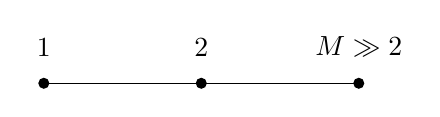
\begin{tikzpicture}
\draw (0,0)--(2,0)--(4,0);
\foreach \x/\lab in {0/1,2/2,4/{M\gg2}}{\fill (\x,0) circle (2pt);\node[above=6pt] at (\x,0){$\lab$};}
\end{tikzpicture}\par\small 图13.1
\end{center}
若将择劣删除贪心算法用于最大化问题，或将择优加入贪心算法用于最小化问题，则比值
\[\frac{G(E,\F,c)}{\operatorname{OPT}(E,\F,c)}\]
不存在正的统一下界或有限的统一上界。只需对图13.1所示简单图，考虑求最大权极小顶点覆盖，或最小权极大稳定集。

但对于拟阵，使用哪一种贪心算法并无区别：由于所有基的基数相同，$(E,\F,c)$ 的最小化问题等价于 $(E,\F,c')$ 的最大化问题，其中 $c'(e):=M-c(e)$，$M:=1+\max\{c(e):e\in E\}$。因此 Kruskal 算法（第6.1节）能最优地求解最小生成树问题。

Edmonds--Rado 定理13.20还给出了最大化问题中最优 $k$ 元解的如下刻画。
\st{定理13.23} 设 $(E,\F)$ 是拟阵，$c:E\to\R$，$k\in\N$，$X\in\F$ 且 $|X|=k$。则 $c(X)=\max\{c(Y):Y\in\F,|Y|=k\}$ 当且仅当以下两个条件成立：
\begin{enumerate}[label=(\alph*)]
\item 对所有满足 $X\cup\{y\}\notin\F$ 的 $y\in E\setminus X$ 以及所有 $x\in C(X,y)$，有 $c(x)\ge c(y)$；
\end{enumerate}

\srcpage{308}
\begin{enumerate}[label=(\alph*),start=2]
\item 对所有满足 $X\cup\{y\}\in\F$ 的 $y\in E\setminus X$ 以及所有 $x\in X$，有 $c(x)\ge c(y)$。
\end{enumerate}
\pr 必要性显然：若某个 $y,x$ 违反其中一个条件，则 $k$ 元集 $X':=(X\cup\{y\})\setminus\{x\}\in\F$ 的费用大于 $X$。
证明充分性。令 $\F':=\{F\in\F:|F|\le k\}$，并令所有 $e\in E$ 的 $c'(e):=c(e)+M$，其中 $M=\max\{|c(e)|:e\in E\}$。将 $E=\{e_1,\ldots,e_n\}$ 排序，使 $c'(e_1)\ge\cdots\ge c'(e_n)$，且对任意 $i$，若 $c'(e_i)=c'(e_{i+1})$、$e_{i+1}\in X$，则 $e_i\in X$（即相同权重中 $X$ 的元素优先）。

设 $X'$ 是按此顺序对实例 $(E,\F',c')$ 运行择优加入贪心算法所得的解。由于 $(E,\F')$ 是拟阵，由定理13.20，
\begin{align*}
c(X')+kM&=c'(X')=\max\{c'(Y):Y\in\F'\}\\
&=\max\{c(Y):Y\in\F,|Y|=k\}+kM.
\end{align*}
最后证明 $X=X'$。已知 $|X|=k=|X'|$。若不同，取 $e_i\in X'\setminus X$，使 $i$ 最小。则 $X\cap\{e_1,\ldots,e_{i-1}\}=X'\cap\{e_1,\ldots,e_{i-1}\}$。若 $X\cup\{e_i\}\notin\F$，由(a)得 $C(X,e_i)\subseteq X'$，矛盾。若 $X\cup\{e_i\}\in\F$，由(b)得 $X\subseteq X'$，也不可能。\qed
第13.7节将用到此定理。$(E,\F)$ 是图拟阵且 $k=r(E)$ 的特例，是定理6.2的一部分。
\sect{13.5\quad 拟阵交}
\st{定义13.24} 给定两个独立系统 $(E,\F_1)$ 和 $(E,\F_2)$，定义它们的\textbf{交}为 $(E,\F_1\cap\F_2)$。
有限个独立系统之交可类似定义。显然所得仍是独立系统。
\st{命题13.25} 任意独立系统 $(E,\F)$ 都是有限个拟阵之交。
\pr 由定理13.12，$(E,\F)$ 的每个回路 $C$ 都定义一个拟阵 $(E,\{F\subseteq E:C\setminus F\ne\varnothing\})$。这些拟阵之交当然就是 $(E,\F)$。\qed
因为拟阵之交一般不是拟阵，不能期望用贪心算法求得最优公共独立集。但下述结论结合定理13.19，可以界定择优加入贪心算法所得解的质量。
\st{命题13.26} 若 $(E,\F)$ 是 $p$ 个拟阵之交，则 $q(E,\F)\ge1/p$。
\srcpage{309}
\pr 由定理13.12(b)，对任意 $X\in\F$ 和 $e\in E$，$X\cup\{e\}$ 至多包含 $p$ 个回路。现由定理13.8即得结论。\qed
由两个拟阵之交构成的独立系统尤其值得关注。首要例子是二分图 $G=(A\mathbin{\dot\cup}B,E(G))$ 中的匹配问题。若 $E=E(G)$，$\F:=\{F\subseteq E:F\text{ 是 }G\text{ 中的匹配}\}$，则 $(E,\F)$ 是两个拟阵之交。具体地，令
\[\F_1:=\{F\subseteq E:|\delta_F(x)|\le1\text{ 对所有 }x\in A\},\]
\[\F_2:=\{F\subseteq E:|\delta_F(x)|\le1\text{ 对所有 }x\in B\}.\]
由命题13.4(d)，$(E,\F_1)$、$(E,\F_2)$ 都是拟阵。显然 $\F=\F_1\cap\F_2$。

第二个例子是由有向图 $G$ 的所有分支构成的独立系统（第13.1节开头的例8）。其中一个拟阵包含每个顶点至多有一条入边的全部边集（见命题13.4(e)），另一个拟阵则是底层无向图的圈拟阵 $M(G)$。

现在描述 Edmonds 用来求解以下问题的算法。
\alg{拟阵交问题}
\textbf{实例：}由独立性预言机给出的两个拟阵 $(E,\F_1)$、$(E,\F_2)$。\par
\textbf{任务：}求 $F\in\F_1\cap\F_2$，使 $|F|$ 最大。

从下述引理开始。回忆：对 $X\in\F$、$e\in E$，若 $X\cup\{e\}\notin\F$，$C(X,e)$ 表示其中唯一的回路；否则 $C(X,e)=\varnothing$。
\st{引理13.27（Frank [1981]）} 设 $(E,\F)$ 是拟阵，$X\in\F$。设 $x_1,\ldots,x_s\in X$，$y_1,\ldots,y_s\notin X$，满足：
\begin{enumerate}[label=(\alph*)]
\item 对 $k=1,\ldots,s$，$x_k\in C(X,y_k)$；
\item 对 $1\le j<k\le s$，$x_j\notin C(X,y_k)$。
\end{enumerate}
则 $(X\setminus\{x_1,\ldots,x_s\})\cup\{y_1,\ldots,y_s\}\in\F$。
\pr 令 $X_r:=(X\setminus\{x_1,\ldots,x_r\})\cup\{y_1,\ldots,y_r\}$，归纳证明所有 $X_r\in\F$。$r=0$ 显然。假设 $X_{r-1}\in\F$。若 $X_{r-1}\cup\{y_r\}\in\F$，立即得 $X_r\in\F$；否则由定理13.12(b)，$X_{r-1}\cup\{y_r\}$ 包含唯一回路 $C$。由(b)，$C(X,y_r)\subseteq X_{r-1}\cup\{y_r\}$，所以 $C=C(X,y_r)$。再由(a)，$x_r\in C$，故 $X_r=(X_{r-1}\cup\{y_r\})\setminus\{x_r\}\in\F$。\qed
Edmonds 拟阵交算法的思想如下：从 $X=\varnothing$ 出发，每次迭代使 $X$ 增加一个元素。一般不能指望存在 $e$ 使 $X\cup\{e\}\in\F_1\cap\F_2$，因此寻找“交错路”。为此定义辅助图。将 $C(X,e)$ 用于 $(E,\F_i)$ 时记作 $C_i(X,e)$（$i=1,2$）。

\srcpage{310}
\begin{center}
\begin{tikzpicture}[>=Stealth,scale=.82]
\draw (0,0) ellipse (.48 and 2.15);\draw (3.5,0) ellipse (.48 and 2.15);
\node at (0,2.5){$X$};\node at (3.5,2.5){$E\setminus X$};
\foreach \y in {.55,1.6}{\draw[->](3.5,\y)--(0,\y);}
\foreach \y in {-.55,-1.6}{\draw[->](0,\y)--(3.5,\y);}
\draw (3.1,1.05)--(3.9,1.05);\draw(3.1,-1.05)--(3.9,-1.05);
\node at (4.25,1.6){$S_X$};\node at (4.25,-1.6){$T_X$};
\node at (1.75,1.05){$A_X^{(2)}$};\node at (1.75,-1.05){$A_X^{(1)}$};
\end{tikzpicture}\par\small 图13.2
\end{center}
给定 $X\in\F_1\cap\F_2$，定义有向辅助图 $G_X$：
\begin{align*}
A_X^{(1)}&:=\{(x,y):y\in E\setminus X,\ x\in C_1(X,y)\setminus\{y\}\},\\
A_X^{(2)}&:=\{(y,x):y\in E\setminus X,\ x\in C_2(X,y)\setminus\{y\}\},\\
G_X&:=(E,A_X^{(1)}\cup A_X^{(2)}).
\end{align*}
令
\[S_X:=\{y\in E\setminus X:X\cup\{y\}\in\F_1\},\qquad
T_X:=\{y\in E\setminus X:X\cup\{y\}\in\F_2\},\]
见图13.2，并寻找从 $S_X$ 到 $T_X$ 的最短路。这样的路使我们能够扩充 $X$。（若 $S_X\cap T_X\ne\varnothing$，就有长度为0的路，可将交集中的任一元素加入 $X$。）
\st{引理13.28} 设 $X\in\F_1\cap\F_2$。设 $y_0,x_1,y_1,\ldots,x_s,y_s$ 依次为 $G_X$ 中一条最短 $y_0$--$y_s$ 路的顶点，且 $y_0\in S_X$、$y_s\in T_X$。则
\[X':=(X\cup\{y_0,\ldots,y_s\})\setminus\{x_1,\ldots,x_s\}\in\F_1\cap\F_2.\]
\pr 首先说明 $X\cup\{y_0\}$、$x_1,\ldots,x_s$ 和 $y_1,\ldots,y_s$ 对 $\F_1$ 满足引理13.27。因为 $y_0\in S_X$，有 $X\cup\{y_0\}\in\F_1$。因所有 $(x_j,y_j)\in A_X^{(1)}$，(a)成立；(b)也成立，否则可对路取捷径。因此 $X'\in\F_1$。
其次，$X\cup\{y_s\}$、$x_s,x_{s-1},\ldots,x_1$ 和 $y_{s-1},\ldots,y_1,y_0$ 对 $\F_2$ 满足引理13.27。因为 $y_s\in T_X$，有 $X\cup\{y_s\}\in\F_2$。因所有 $(y_{j-1},x_j)\in A_X^{(2)}$，(a)成立；而(b)成立，因为否则可对路取捷径。

\srcpage{311}
所以 $X'\in\F_2$。\qed
下面证明：若 $G_X$ 中没有 $S_X$--$T_X$ 路，则 $X$ 已经具有最大基数。需要以下简单事实。
\st{命题13.29} 设 $(E,\F_1)$、$(E,\F_2)$ 是两个拟阵，秩函数分别为 $r_1,r_2$。则对任意 $F\in\F_1\cap\F_2$、$Q\subseteq E$，
\[|F|\le r_1(Q)+r_2(E\setminus Q).\]
\pr $F\cap Q\in\F_1$ 蕴含 $|F\cap Q|\le r_1(Q)$；同样 $F\setminus Q\in\F_2$ 蕴含 $|F\setminus Q|\le r_2(E\setminus Q)$。两式相加即得。\qed
\st{引理13.30} $X\in\F_1\cap\F_2$ 的基数最大，当且仅当 $G_X$ 中不存在 $S_X$--$T_X$ 路。
\pr 若存在这样的路，则也存在最短的一条。应用引理13.28，即得基数更大的 $X'\in\F_1\cap\F_2$。
\begin{center}
\begin{tikzpicture}[>=Stealth,scale=.82]
\draw (0,0) ellipse (.48 and 2.15);\draw (3.5,0) ellipse (.48 and 2.15);
\node at(0,2.5){$X$};\node at(3.5,2.5){$E\setminus X$};
\foreach \y in {.55,1.6}{\draw[->](3.5,\y)--(0,\y);}
\foreach \y in {-.55,-1.6}{\draw[->](0,\y)--(3.5,\y);}
\draw[->](3.5,-.15)--(0,1.05);\draw[->](0,-1.05)--(3.5,.85);
\draw(3.1,1.05)--(3.9,1.05);\draw(3.1,-1.05)--(3.9,-1.05);
\draw[dashed](-1.1,-.32)--(4.6,.32);
\node at(-.85,0){$R$};\node at(-.9,-.62){$E\setminus R$};
\node at(4.25,1.6){$S_X$};\node at(4.25,-1.6){$T_X$};
\node at(1.75,1.05){$A_X^{(2)}$};\node at(1.75,-1.05){$A_X^{(1)}$};
\end{tikzpicture}\par\small 图13.3
\end{center}
否则，设 $R$ 是 $G_X$ 中从 $S_X$ 可达的顶点集（见图13.3），则 $R\cap T_X=\varnothing$。以 $r_1,r_2$ 分别表示 $\F_1,\F_2$ 的秩函数。
断言 $r_2(R)=|X\cap R|$。否则存在 $y\in R\setminus X$，使 $(X\cap R)\cup\{y\}\in\F_2$。由于 $y\notin T_X$，$X\cup\{y\}\notin\F_2$，所以回路 $C_2(X,y)$ 必包含某个 $x\in X\setminus R$。但 $(y,x)\in A_X^{(2)}$ 意味着有边离开 $R$，与 $R$ 的定义矛盾。

\srcpage{312}
再证 $r_1(E\setminus R)=|X\setminus R|$。否则存在 $y\in(E\setminus R)\setminus X$，使 $(X\setminus R)\cup\{y\}\in\F_1$。由于 $y\notin S_X$，$X\cup\{y\}\notin\F_1$，所以回路 $C_1(X,y)$ 必包含某个 $x\in X\cap R$。但 $(x,y)\in A_X^{(1)}$ 意味着有边离开 $R$，与 $R$ 的定义矛盾。
综上，$|X|=r_2(R)+r_1(E\setminus R)$。由命题13.29，$X$ 最优。\qed
这一证明的最后部分给出如下极小极大等式。
\st{定理13.31（Edmonds [1970]）} 设 $(E,\F_1)$、$(E,\F_2)$ 是两个拟阵，其秩函数为 $r_1,r_2$。则
\[\max\{|X|:X\in\F_1\cap\F_2\}=\min\{r_1(Q)+r_2(E\setminus Q):Q\subseteq E\}.\quad\square\]
现在可以详细描述算法。
\alg{Edmonds 拟阵交算法}
\textbf{输入：}由独立性预言机给出的两个拟阵 $(E,\F_1)$、$(E,\F_2)$。\par
\textbf{输出：}基数最大的集合 $X\in\F_1\cap\F_2$。
\begin{enumerate}[label=\arabic*.]
\item 令 $X:=\varnothing$。
\item 对每个 $y\in E\setminus X$ 和 $i\in\{1,2\}$，计算
\[C_i(X,y):=\{x\in X\cup\{y\}:X\cup\{y\}\notin\F_i,\ (X\cup\{y\})\setminus\{x\}\in\F_i\}.\]
\item 按前面的定义计算 $S_X,T_X,G_X$。
\item 用广度优先搜索（BFS）在 $G_X$ 中寻找最短 $S_X$--$T_X$ 路 $P$。若不存在则停止。
\item 令 $X:=X\mathbin{\triangle}V(P)$，返回步骤2。
\end{enumerate}
\st{定理13.32} Edmonds 拟阵交算法在 $O(|E|^3\theta)$ 时间内正确求解拟阵交问题，其中 $\theta$ 是两种独立性预言机复杂度的最大值。
\pr 正确性来自引理13.28、13.30。步骤2、3可在 $O(|E|^2\theta)$ 时间内完成，步骤4可在 $O(|E|)$ 时间内完成。由于增广次数至多 $|E|$，总复杂度为 $O(|E|^3\theta)$。\qed
Cunningham [1986] 及 Gabow 和 Xu [1996] 讨论了更快的拟阵交算法。顺便指出：在三个拟阵之交中寻找最大基数集合是 NP 困难问题，见第15章习题14(c)。

\srcpage{313}
\sect{13.6\quad 拟阵划分}
现在不再考虑拟阵的交，而考虑按如下方式定义的并。
\st{定义13.33} 设 $(E,\F_1),\ldots,(E,\F_k)$ 是 $k$ 个拟阵。若存在划分 $X=X_1\mathbin{\dot\cup}\cdots\mathbin{\dot\cup}X_k$，使 $X_i\in\F_i$（$i=1,\ldots,k$），则称 $X\subseteq E$ \textbf{可划分}。令 $\F$ 为 $E$ 的可划分子集族，则称 $(E,\F)$ 为这些拟阵的\textbf{并}或\textbf{和}。
我们将证明拟阵的并仍是拟阵，并通过拟阵交求解下列问题。
\alg{拟阵划分问题}
\textbf{实例：}数 $k\in\N$，以及由独立性预言机给出的 $k$ 个拟阵 $(E,\F_1),\ldots,(E,\F_k)$。\par
\textbf{任务：}求基数最大的可划分集合 $X\subseteq E$。
关于拟阵划分的主要定理是：
\st{定理13.34（Nash-Williams [1967]）} 设 $(E,\F_1),\ldots,(E,\F_k)$ 是拟阵，其秩函数为 $r_1,\ldots,r_k$；设 $(E,\F)$ 是它们的并。则 $(E,\F)$ 是拟阵，其秩函数为
\[r(X)=\min_{A\subseteq X}\left(|X\setminus A|+\sum_{i=1}^kr_i(A)\right).\]
\pr $(E,\F)$ 显然是独立系统。设 $X\subseteq E$，先证明上述秩公式。任取可划分的 $Y\subseteq X$，即 $Y=Y_1\mathbin{\dot\cup}\cdots\mathbin{\dot\cup}Y_k$ 且 $Y_i\in\F_i$，以及任意 $A\subseteq X$，都有
\[|Y|=|Y\setminus A|+|Y\cap A|\le|X\setminus A|+\sum_{i=1}^k|Y_i\cap A|
\le|X\setminus A|+\sum_{i=1}^kr_i(A).\]
所以 $r(X)\le\min_{A\subseteq X}(|X\setminus A|+\sum_i r_i(A))$。

另一方面，令 $X':=X\times\{1,\ldots,k\}$，在其上定义两个拟阵。对 $Q\subseteq X'$ 和 $i\in\{1,\ldots,k\}$，记 $Q_i:=\{e\in X:(e,i)\in Q\}$。令
\[\mathcal I_1:=\{Q\subseteq X':Q_i\in\F_i\text{ 对所有 }i=1,\ldots,k\},\]
\[\mathcal I_2:=\{Q\subseteq X':Q_i\cap Q_j=\varnothing\text{ 对所有 }i\ne j\}.\]
显然 $(X',\mathcal I_1)$ 和 $(X',\mathcal I_2)$ 都是拟阵，其秩函数分别为
\[s_1(Q):=\sum_{i=1}^kr_i(Q_i),\qquad s_2(Q):=\left|\bigcup_{i=1}^kQ_i\right|\quad(Q\subseteq X').\]

\srcpage{314}
现在 $X$ 的可划分子集族可写成
\[\{A\subseteq X:\text{存在 }f:A\to\{1,\ldots,k\},\ \{(e,f(e)):e\in A\}\in\mathcal I_1\cap\mathcal I_2\}.\]
所以可划分集合的最大基数，等于 $\mathcal I_1$ 和 $\mathcal I_2$ 中公共独立集的最大基数。由定理13.31，该值为 $\min\{s_1(Q)+s_2(X'\setminus Q):Q\subseteq X'\}$。若 $Q$ 达到此最小值，令 $A:=Q_1\cap\cdots\cap Q_k$，则
\begin{align*}
r(X)&=s_1(Q)+s_2(X'\setminus Q)\\
&=\sum_{i=1}^kr_i(Q_i)+\left|X\setminus\bigcap_{i=1}^kQ_i\right|
\ge\sum_{i=1}^kr_i(A)+|X\setminus A|.
\end{align*}
于是找到了满足 $\sum_i r_i(A)+|X\setminus A|\le r(X)$ 的 $A\subseteq X$。

证明秩公式后，最后证明 $r$ 次模；由定理13.10即知 $(E,\F)$ 是拟阵。设 $X,Y\subseteq E$，取 $A\subseteq X$、$B\subseteq Y$，满足 $r(X)=|X\setminus A|+\sum_i r_i(A)$、$r(Y)=|Y\setminus B|+\sum_i r_i(B)$。则
\begin{align*}
r(X)+r(Y)&=|X\setminus A|+|Y\setminus B|+\sum_{i=1}^k(r_i(A)+r_i(B))\\
&\ge|(X\cup Y)\setminus(A\cup B)|+|(X\cap Y)\setminus(A\cap B)|\\
&\quad+\sum_{i=1}^k(r_i(A\cup B)+r_i(A\cap B))\\
&\ge r(X\cup Y)+r(X\cap Y).
\end{align*}\qed
上述证明中的构造（Edmonds [1970]）将拟阵划分问题归约为拟阵交问题。反向归约也能做到（习题20），所以可把二者看作等价问题。

注意，我们能在任意多个拟阵的并中寻找最大独立集，而超过两个拟阵的交则难以处理。
\sect{13.7\quad 带权拟阵交}
现在将上述算法推广到带权情形。
\alg{带权拟阵交问题}
\textbf{实例：}由独立性预言机给出的两个拟阵 $(E,\F_1)$、$(E,\F_2)$；权函数 $c:E\to\R$。\par
\textbf{任务：}求 $X\in\F_1\cap\F_2$，使其权重 $c(X)$ 最大。

\srcpage{315}
下面描述 Frank [1981] 的原始对偶算法，它推广了 Edmonds 拟阵交算法。仍从 $X:=X_0=\varnothing$ 出发，每次迭代使基数增加1，得到 $X_0,\ldots,X_m\in\F_1\cap\F_2$，满足 $|X_k|=k$（$k=0,\ldots,m$），其中 $m=\max\{|X|:X\in\F_1\cap\F_2\}$。每个 $X_k$ 都将最优，即
\[c(X_k)=\max\{c(X):X\in\F_1\cap\F_2,|X|=k\}.\tag{13.4}\]
所以最终只需在 $X_0,\ldots,X_m$ 中选择最优集合。

主要思想是分拆权函数。任意阶段都有 $c_1,c_2:E\to\R$，使所有 $e\in E$ 满足 $c_1(e)+c_2(e)=c(e)$。对每个 $k$，保证
\[c_i(X_k)=\max\{c_i(X):X\in\F_i,|X|=k\}\quad(i=1,2).\tag{13.5}\]
该条件显然蕴含(13.4)。为得到(13.5)，使用定理13.23的最优性准则。只考虑 $G_X$ 的子图 $\overline G$，以及 $S_X,T_X$ 的子集 $\overline S,\overline T$。
\alg{带权拟阵交算法}
\textbf{输入：}由独立性预言机给出的拟阵 $(E,\F_1)$、$(E,\F_2)$；权函数 $c:E\to\R$。\par
\textbf{输出：}最大权集合 $X\in\F_1\cap\F_2$。
\begin{enumerate}[label=\arabic*.]
\item 令 $k:=0$、$X_0:=\varnothing$，对所有 $e\in E$ 令 $c_1(e):=c(e)$、$c_2(e):=0$。
\item 对每个 $y\in E\setminus X_k$ 及 $i\in\{1,2\}$，计算
\[C_i(X_k,y):=\{x\in X_k\cup\{y\}:X_k\cup\{y\}\notin\F_i,\ (X_k\cup\{y\})\setminus\{x\}\in\F_i\}.\]
\item 计算
\begin{align*}
A^{(1)}&:=\{(x,y):y\in E\setminus X_k,x\in C_1(X_k,y)\setminus\{y\}\},\\
A^{(2)}&:=\{(y,x):y\in E\setminus X_k,x\in C_2(X_k,y)\setminus\{y\}\},\\
S&:=\{y\in E\setminus X_k:X_k\cup\{y\}\in\F_1\},\\
T&:=\{y\in E\setminus X_k:X_k\cup\{y\}\in\F_2\}.
\end{align*}
\item 计算
\begin{align*}
m_1&:=\max\{c_1(y):y\in S\},&m_2&:=\max\{c_2(y):y\in T\},\\
\overline S&:=\{y\in S:c_1(y)=m_1\},&\overline T&:=\{y\in T:c_2(y)=m_2\},\\
\overline A^{(1)}&:=\{(x,y)\in A^{(1)}:c_1(x)=c_1(y)\},\\
\overline A^{(2)}&:=\{(y,x)\in A^{(2)}:c_2(x)=c_2(y)\},\\
\overline G&:=(E,\overline A^{(1)}\cup\overline A^{(2)}).
\end{align*}
\end{enumerate}

\srcpage{316}
\begin{enumerate}[label=\arabic*.,start=5]
\item 用 BFS 计算 $\overline G$ 中从 $\overline S$ 可达的顶点集 $R$。
\item 若 $R\cap\overline T\ne\varnothing$：在 $\overline G$ 中找一条边数最少的 $\overline S$--$\overline T$ 路 $P$，令 $X_{k+1}:=X_k\mathbin{\triangle}V(P)$、$k:=k+1$，返回步骤2。
\item 计算
\begin{align*}
\varepsilon_1&:=\min\{c_1(x)-c_1(y):(x,y)\in A^{(1)}\cap\delta^+(R)\},\\
\varepsilon_2&:=\min\{c_2(x)-c_2(y):(y,x)\in A^{(2)}\cap\delta^+(R)\},\\
\varepsilon_3&:=\min\{m_1-c_1(y):y\in S\setminus R\},\\
\varepsilon_4&:=\min\{m_2-c_2(y):y\in T\cap R\},\\
\varepsilon&:=\min\{\varepsilon_1,\varepsilon_2,\varepsilon_3,\varepsilon_4\},
\end{align*}
其中约定 $\min\varnothing:=\infty$。
\item 若 $\varepsilon<\infty$：对所有 $x\in R$ 令 $c_1(x):=c_1(x)-\varepsilon$、$c_2(x):=c_2(x)+\varepsilon$，返回步骤4。若 $\varepsilon=\infty$：在 $X_0,X_1,\ldots,X_k$ 中选权重最大的一个，记为 $X$，停止。
\end{enumerate}
该算法的早期版本见 Edmonds [1979] 和 Lawler [1976]。
\st{定理13.35（Frank [1981]）} 带权拟阵交算法在 $O(|E|^4+|E|^3\theta)$ 时间内正确求解带权拟阵交问题，其中 $\theta$ 是两种独立性预言机复杂度的最大值。
\pr 设 $m$ 是 $k$ 的最终值。算法计算 $X_0,X_1,\ldots,X_m$。先对 $k$ 归纳证明 $X_k\in\F_1\cap\F_2$。$k=0$ 显然。若当前 $X_k\in\F_1\cap\F_2$，则 $\overline G$ 是 $(E,A^{(1)}\cup A^{(2)})=G_{X_k}$ 的子图。所以当步骤5中找到路 $P$ 时，引理13.28保证 $X_{k+1}\in\F_1\cap\F_2$。
算法停止时，$\varepsilon_1=\varepsilon_2=\varepsilon_3=\varepsilon_4=\infty$，所以 $G_{X_m}$ 中不能从 $S$ 到达 $T$。由引理13.30，$m=|X_m|=\max\{|X|:X\in\F_1\cap\F_2\}$。

为证正确性，证明每个 $k=0,\ldots,m$ 都满足 $c(X_k)=\max\{c(X):X\in\F_1\cap\F_2,|X|=k\}$。因始终 $c=c_1+c_2$，只需证明算法任意阶段都满足(13.5)。初始 $k=0$ 时显然；利用定理13.23证明其永不被破坏。

步骤6令 $X_{k+1}:=X_k\mathbin{\triangle}V(P)$ 时，设 $P$ 是 $s$--$t$ 路，$s\in\overline S$、$t\in\overline T$。由 $\overline G$ 的定义，$c_1(X_{k+1})=c_1(X_k)+c_1(s)$，$c_2(X_{k+1})=c_2(X_k)+c_2(t)$。因 $X_k$ 满足(13.5)，定理13.23(a)、(b)对 $X_k$ 和每个 $\F_i$ 都成立。
由 $\overline S$ 的定义，两条件对 $X_k\cup\{s\}$ 和 $\F_1$ 继续成立。所以 $c_1(X_{k+1})=c_1(X_k\cup\{s\})=\max\{c_1(Y):Y\in\F_1,|Y|=k+1\}$。同理由 $\overline T$ 的定义，两条件对 $X_k\cup\{t\}$ 和 $\F_2$ 继续成立。

\srcpage{317}
于是 $c_2(X_{k+1})=c_2(X_k\cup\{t\})=\max\{c_2(Y):Y\in\F_2,|Y|=k+1\}$。换言之，$X_{k+1}$ 确实满足(13.5)。

现在考虑步骤8改变 $c_1,c_2$ 的情形。先证 $\varepsilon>0$。由(13.5)及定理13.23，对所有 $y\in E\setminus X_k$、$x\in C_1(X_k,y)\setminus\{y\}$，有 $c_1(x)\ge c_1(y)$。故任意 $(x,y)\in A^{(1)}$ 均满足该不等式。又由 $R$ 的定义，$\delta^+(R)$ 中没有边属于 $\overline A^{(1)}$，所以 $\varepsilon_1>0$。同理 $\varepsilon_2>0$。对所有 $y\in S$，有 $m_1\ge c_1(y)$；若还满足 $y\notin R$，则 $y\notin\overline S$，所以 $m_1>c_1(y)$。故 $\varepsilon_3>0$。利用 $\overline T\cap R=\varnothing$，同理得 $\varepsilon_4>0$。因此 $\varepsilon>0$。

下面证明步骤8保持(13.5)。以 $c'_1$ 表示修改后的 $c_1$，即 $c'_1(x)=c_1(x)-\varepsilon$（$x\in R$），否则不变。证明 $X_k,c'_1$ 对 $\F_1$ 满足定理13.23。

为证(a)，取 $y\in E\setminus X_k$、$x\in C_1(X_k,y)\setminus\{y\}$。若 $c'_1(x)<c'_1(y)$，因 $c_1(x)\ge c_1(y)$ 且 $\varepsilon>0$，必有 $x\in R$、$y\notin R$。又因 $(x,y)\in A^{(1)}$，有
\[\varepsilon\le\varepsilon_1\le c_1(x)-c_1(y)=(c'_1(x)+\varepsilon)-c'_1(y),\]
矛盾。为证(b)，取 $x\in X_k$、$y\in E\setminus X_k$ 且 $X_k\cup\{y\}\in\F_1$。若 $c'_1(y)>c'_1(x)$，因 $c_1(y)\le m_1\le c_1(x)$，必有 $x\in R$、$y\notin R$。又因 $y\in S$，
\[\varepsilon\le\varepsilon_3\le m_1-c_1(y)\le c_1(x)-c_1(y)=(c'_1(x)+\varepsilon)-c'_1(y),\]
矛盾。

以 $c'_2$ 表示修改后的 $c_2$，即 $c'_2(x)=c_2(x)+\varepsilon$（$x\in R$），否则不变。证明 $X_k,c'_2$ 对 $\F_2$ 满足定理13.23。
为证(a)，取 $y\in E\setminus X_k$、$x\in C_2(X_k,y)\setminus\{y\}$。若 $c'_2(x)<c'_2(y)$，因 $c_2(x)\ge c_2(y)$，必有 $y\in R$、$x\notin R$。又因 $(y,x)\in A^{(2)}$，
\[\varepsilon\le\varepsilon_2\le c_2(x)-c_2(y)=c'_2(x)-(c'_2(y)-\varepsilon),\]
矛盾。为证(b)，取 $x\in X_k$、$y\in E\setminus X_k$ 且 $X_k\cup\{y\}\in\F_2$。若 $c'_2(y)>c'_2(x)$，因 $c_2(y)\le m_2\le c_2(x)$，必有 $y\in R$、$x\notin R$。由 $y\in T$，
\[\varepsilon\le\varepsilon_4\le m_2-c_2(y)\le c_2(x)-c_2(y)=c'_2(x)-(c'_2(y)-\varepsilon),\]
矛盾。因此步骤8不破坏(13.5)，算法正确。

下面分析运行时间。注意步骤8之后，在步骤4、5重新计算的 $\overline S,\overline T,R$ 分别是原集合的超集。若 $\varepsilon=\varepsilon_4<\infty$，随后发生增广（$k$ 增加）；否则 $R$ 的基数立即在步骤5中至少增加1。因此两次增广之间，步骤4--8重复少于 $|E|$ 次。
步骤4--8的时间为 $O(|E|^2)$，故两次增广之间总时间为 $O(|E|^3)$，另加步骤2中的 $O(|E|^2)$ 次预言机调用。因增广次数 $m\le|E|$，得到所述总运行时间。\qed
运行时间容易改进到 $O(|E|^3\theta)$（习题22）。
\srcpage{318}
\sect{第13章习题}
\begin{enumerate}[label=\arabic*.]
\item 证明第13.1节开头列表中，除(5)、(6)外的所有独立系统一般都不是拟阵。
\item 证明含4个元素、秩为2的均匀拟阵不是图拟阵。
\item 证明每个图拟阵在每个域上都可表示。
\item 设 $G$ 是无向图，$K\in\N$，$\F$ 包含 $E(G)$ 中所有可写为 $K$ 个森林之并的子集。证明 $(E(G),\F)$ 是拟阵。
\item 对第13.1节开头列出的独立系统，求其秩商的紧下界。
\item 设 $\mathcal S$ 是集合族。若存在双射 $\varphi:T\to\mathcal S$，使所有 $t\in T$ 满足 $t\in\varphi(t)$，则称 $T$ 是 $\mathcal S$ 的\textbf{横截集}（transversal）。（横截集存在的充要条件见第10章习题6。）假定 $\mathcal S$ 有横截集，证明其横截集族是某个拟阵的基族。
\item 设 $E$ 是有限集，$\B\subseteq2^E$。证明 $\B$ 是某个拟阵 $(E,\F)$ 的基集合，当且仅当：\par
(B1) $\B\ne\varnothing$；\par
(B2) 对任意 $B_1,B_2\in\B$ 和 $y\in B_2\setminus B_1$，存在 $x\in B_1\setminus B_2$，使 $(B_1\setminus\{x\})\cup\{y\}\in\B$。
\item 设 $G$ 是图。令 $\F$ 为满足以下条件的集合 $X\subseteq V(G)$ 的全体：存在一个最大匹配，它不覆盖 $X$ 中任何顶点。证明 $(V(G),\F)$ 是拟阵。其对偶拟阵是什么？
\item 将定理13.16推广到非连通图 $G$，证明仍有 $M(G^*)=(M(G))^*$。\par
\textbf{提示：}使用第2章习题31(a)。
\item 证明第13.3节列表中的杂族(3)、(6)具有最大流最小割性质（使用定理19.10）。证明杂族(1)、(4)、(5)不具有该性质。
\item[$11.^*$] 若对任意奇数 $k$ 和 $X_1,\ldots,X_k\in\F$，都存在 $Y\in\F$ 使 $Y\subseteq X_1\triangle\cdots\triangle X_k$，则称杂族 $(E,\F)$ 为\textbf{二元杂族}。证明极小 $T$-连接杂族和极小 $T$-割杂族（第13.3节例(7)）都是二元的。证明杂族二元当且仅当对所有 $A\in\F$ 及 $B\in\F^*$，$|A\cap B|$ 都是奇数，其中 $(E,\F^*)$ 是阻塞杂族。由此推出：杂族二元当且仅当其阻塞杂族二元。\par
\textbf{注：}Seymour [1977] 对具有最大流最小割性质的二元杂族作了分类。
\item[$12.^*$] 设 $P$ 是阻塞型多面体，即对所有 $x\in P$、$y\ge0$，有 $x+y\in P$。定义其阻塞多面体为 $B(P):=\{z:z^\top x\ge1\text{ 对所有 }x\in P\}$。证明 $B(P)$ 仍是阻塞型多面体，且 $B(B(P))=P$。\par
\textbf{注：}与定理4.22比较。
\setcounter{enumi}{12}
\item 如何在多项式时间内检验：完全图 $G$ 的给定边集是否为 $G$ 中某个哈密顿回路的子集？
\end{enumerate}

\srcpage{319}
\begin{enumerate}[label=\arabic*.,start=14]
\item 证明若 $(E,\F)$ 是拟阵，则择优加入贪心算法能在基族上最大化任意瓶颈函数 $c(F)=\min\{c_e:e\in F\}$。
\item 设 $(E,\F)$ 是拟阵，$c:E\to\R$，任意 $e\ne e'$ 都有 $c(e)\ne c(e')$，且所有 $e$ 满足 $c(e)\ne0$。证明 $(E,\F,c)$ 的最大化问题和最小化问题各有唯一最优解。
\item[$16.^*$] 证明对拟阵，独立性预言机、基超集预言机、闭包预言机和秩预言机在多项式意义下等价。\par
\textbf{提示：}将秩预言机归约到独立性预言机时，使用择优加入贪心算法；将独立性预言机归约到基超集预言机时，使用择劣删除贪心算法。（Hausmann 和 Korte [1981]）
\setcounter{enumi}{16}
\item 给定无向图 $G$，希望用最少颜色给边着色，使 $G$ 的每个圈 $C$ 的边不全同色。证明该问题有多项式时间算法。
\item 设 $(E,\F_1),\ldots,(E,\F_k)$ 是拟阵，秩函数为 $r_1,\ldots,r_k$。证明 $X\subseteq E$ 可划分，当且仅当对所有 $A\subseteq X$，$|A|\le\sum_{i=1}^kr_i(A)$。说明定理6.19是其特例。（Edmonds 和 Fulkerson [1965]）
\item 设 $(E,\F)$ 是拟阵，秩函数为 $r$。利用定理13.34证明：
\begin{enumerate}[label=(\alph*)]
\item $(E,\F)$ 有 $k$ 个两两不交的基，当且仅当对所有 $A\subseteq E$，$kr(A)+|E\setminus A|\ge kr(E)$。
\item $(E,\F)$ 有 $k$ 个独立集，其并为 $E$，当且仅当对所有 $A\subseteq E$，$kr(A)\ge|A|$。
\end{enumerate}
说明定理6.19和6.16是其特例。
\item 设 $(E,\F_1)$、$(E,\F_2)$ 是拟阵。设 $X$ 是关于 $(E,\F_1)$、$(E,\F_2^*)$ 的极大可划分子集：$X=X_1\mathbin{\dot\cup}X_2$，其中 $X_1\in\F_1$、$X_2\in\F_2^*$。令 $B_2\supseteq X_2$ 是 $\F_2^*$ 的一个基。证明 $X\setminus B_2$ 是 $\F_1\cap\F_2$ 中基数最大的集合。（Edmonds [1970]）
\item 设 $(E,\mathcal S)$ 是集合系统，$(E,\F)$ 是秩函数为 $r$ 的拟阵。证明 $\mathcal S$ 有一个在 $(E,\F)$ 中独立的横截集，当且仅当对所有 $\mathcal B\subseteq\mathcal S$，有 $r(\bigcup_{B\in\mathcal B}B)\ge|\mathcal B|$。\par
\textbf{提示：}先利用定理13.34，描述以所有横截集为独立集的拟阵的秩函数（习题6）；再应用定理13.31。（Rado [1942]）
\item 证明带权拟阵交算法的运行时间（参见定理13.35）可以改进到 $O(|E|^3\theta)$。
\item 设 $(E,\F_1)$、$(E,\F_2)$ 是拟阵，$c:E\to\R$。对每个 $k$，设 $X_k\in\F_1\cap\F_2$，$|X_k|=k$，且 $c(X_k)=\max\{c(X):X\in\F_1\cap\F_2,|X|=k\}$，其中 $k=0,\ldots,m$。证明对 $k=1,\ldots,m-2$，
\[c(X_{k+1})-c(X_k)\le c(X_k)-c(X_{k-1}).\]
（Krogdahl，未发表）
\end{enumerate}

\srcpage{320}
\begin{enumerate}[label=\arabic*.,start=24]
\item 考虑以下问题：给定带边权的有向图 $G$、顶点 $s\in V(G)$ 和数 $K$，求 $G$ 的最小权子图 $H$，使 $H$ 包含从 $s$ 到每个其他顶点的 $K$ 条边不交路。证明此问题可以归约为带权拟阵交问题。\par
\textbf{提示：}见第6章习题18及本章习题4。（Edmonds [1970]；Frank 和 Tardos [1989]；Gabow [1995]）
\item 设 $A,B$ 是基数为 $n\in\N$ 的有限集，$\bar a\in A$，$c:\{\{a,b\}:a\in A,b\in B\}\to\R$ 是费用函数。令 $\mathcal T$ 为所有满足 $V(T)=A\mathbin{\dot\cup}B$ 且对每个 $a\in A\setminus\{\bar a\}$ 有 $|\delta_T(a)|=2$ 的树 $T$ 的边集族。证明可在 $O(n^7)$ 时间内求得 $\mathcal T$ 中费用最小的元素。有多少条边与 $\bar a$ 关联？
\end{enumerate}
\sect{第13章参考文献}
{\small\setlength{\parindent}{0pt}\setlength{\parskip}{5pt}\sloppy
\textbf{一般文献}\par
Bixby, R.E., and Cunningham, W.H. [1995]: Matroid optimization and algorithms. In: Handbook of Combinatorics; Vol. 1 (R.L. Graham, M. Grötschel, L. Lovász, eds.), Elsevier, Amsterdam, 1995\par
Cook, W.J., Cunningham, W.H., Pulleyblank, W.R., and Schrijver, A. [1998]: Combinatorial Optimization. Wiley, New York 1998, Chapter 8\par
Faigle, U. [1987]: Matroids in combinatorial optimization. In: Combinatorial Geometries (N. White, ed.), Cambridge University Press, 1987\par
Gondran, M., and Minoux, M. [1984]: Graphs and Algorithms. Wiley, Chichester 1984, Chapter 9\par
Lawler, E.L. [1976]: Combinatorial Optimization; Networks and Matroids. Holt, Rinehart and Winston, New York 1976, Chapters 7 and 8\par
Oxley, J.G. [1992]: Matroid Theory. Oxford University Press, Oxford 1992\par
von Randow, R. [1975]: Introduction to the Theory of Matroids. Springer, Berlin 1975\par
Recski, A. [1989]: Matroid Theory and its Applications. Springer, Berlin, 1989\par
Schrijver, A. [2003]: Combinatorial Optimization: Polyhedra and Efficiency. Springer, Berlin 2003, Chapters 39–42\par
Welsh, D.J.A. [1976]: Matroid Theory. Academic Press, London 1976\par
\textbf{引用文献}\par
Cunningham, W.H. [1986] : Improved bounds for matroid partition and intersection algorithms. SIAM Journal on Computing 15 (1986), 948–957\par
Edmonds, J. [1970]: Submodular functions, matroids and certain polyhedra. In: Combinatorial Structures and Their Applications; Proceedings of the Calgary International Conference on Combinatorial Structures and Their Applications 1969 (R. Guy, H. Hanani, N. Sauer, J. Schonheim, eds.), Gordon and Breach, New York 1970, pp. 69–87\par
Edmonds, J. [1971]: Matroids and the greedy algorithm. Mathematical Programming 1 (1971), 127–136\par
Edmonds, J. [1979]: Matroid intersection. In: Discrete Optimization I; Annals of Discrete Mathematics 4 (P.L. Hammer, E.L. Johnson, B.H. Korte, eds.), North-Holland, Amsterdam 1979, pp. 39–49\par
Edmonds, J., and Fulkerson, D.R. [1965]: Transversals and matroid partition. Journal of Research of the National Bureau of Standards B 69 (1965), 67–72\par
}

\srcpage{321}
{\small\setlength{\parindent}{0pt}\setlength{\parskip}{5pt}\sloppy
Frank, A. [1981]: A weighted matroid intersection algorithm. Journal of Algorithms 2 (1981), 328–336\par
Frank, A., and Tardos,É. [1989]: An application of submodular flows. Linear Algebra and Its Applications 114/115 (1989), 329–348\par
Fulkerson, D.R. [1971]: Blocking and anti-blocking pairs of polyhedra. Mathematical Programming 1 (1971), 168–194\par
Gabow, H.N. [1995]: A matroid approach to finding edge connectivity and packing arborescences. Journal of Computer and System Sciences 50 (1995), 259–273\par
Gabow, H.N., and Xu, Y. [1996]: Efficient theoretic and practical algorithms for linear matroid intersection problems. Journal of Computer and System Sciences 53 (1996), 129–147\par
Hausmann, D., Jenkyns, T.A., and Korte, B. [1980]: Worst case analysis of greedy type algorithms for independence systems. Mathematical Programming Study 12 (1980), 120– 131\par
Hausmann, D., and Korte, B. [1981]: Algorithmic versus axiomatic definitions of matroids. Mathematical Programming Study 14 (1981), 98–111\par
Jenkyns, T.A. [1976]: The efficiency of the greedy algorithm. Proceedings of the 7th SE Conference on Combinatorics, Graph Theory, and Computing, Utilitas Mathematica, Winnipeg 1976, pp. 341–350\par
Korte, B., and Hausmann, D. [1978]: An analysis of the greedy algorithm for independence systems. In: Algorithmic Aspects of Combinatorics; Annals of Discrete Mathematics 2 (B. Alspach, P. Hell, D.J. Miller, eds.), North-Holland, Amsterdam 1978, pp. 65–74\par
Korte, B., and Monma, C.L. [1979]: Some remarks on a classification of oracle-type algorithms. In: Numerische Methoden bei graphentheoretischen und kombinatorischen Problemen; Band 2 (L. Collatz, G. Meinardus, W. Wetterling, eds.), Birkhäuser, Basel 1979, pp. 195–215\par
Lehman, A. [1979]: On the width-length inequality. Mathematical Programming 17 (1979), 403–417\par
Nash-Williams, C.S.J.A. [1967]: An application of matroids to graph theory. In: Theory of Graphs; Proceedings of an International Symposium in Rome 1966 (P. Rosenstiehl, ed.), Gordon and Breach, New York, 1967, pp. 263–265\par
Rado, R. [1942]: A theorem on independence relations. Quarterly Journal of Math. Oxford 13 (1942), 83–89\par
Rado, R. [1957]: Note on independence functions. Proceedings of the London Mathematical Society 7 (1957), 300–320\par
Seymour, P.D. [1977]: The matroids with the Max-Flow Min-Cut property. Journal of Combinatorial Theory B 23 (1977), 189–222\par
Whitney, H. [1933]: Planar graphs. Fundamenta Mathematicae 21 (1933), 73–84\par
Whitney, H. [1935]: On the abstract properties of linear dependence. American Journal of Mathematics 57 (1935), 509–533\par
}

